In total 18,555 timesteps have been computed, with transient results every 10 timesteps and full backups every 100 timesteps. With a timestep duration of 1e-5 seconds this makes a physical simulation duration of 0.2s. Altough this seems to be a rather short time, it is sufficient, because with a velocity of 66.8m/s the flow passes the wing surface with a length of 1m five times during this simulation time.
\section{Checking border conditions}
The post-processing was conducted with Ansys CFX-Post 15.0. The first thing was checking whether the y+ value on the wing surface was within the correct scope. This was achieved by plotting the y+ value on the wing surface as you can see in figure ?? . The value on the surface in nowhere beyond one, which is a necessary requirement in order to receive reliable values for the heat transfer.

Additionally the drag coefficient of the wing was mirrored over the last timesteps. When it does not change any more over several timesteps, it can be assumed that the simulation has reached a kind of steady state. The value for the drag coefficient was calculated in Ansys CFX-Post by the equation
\begin{equation}
C_D = \frac{F_{horizontal}}{\frac{1}{2} \rho U^2 A_{eff}}
\end{equation}
where Aeff is the projection of the wing geometry in flow direction and Fhorizontal the force operating in x-direction.
The values for the drag coefficient for the last 200 steps are listed in table ??. It can be seen that they stay the same, apart from some minor deviations.
\begin{figure}[h]
\centering
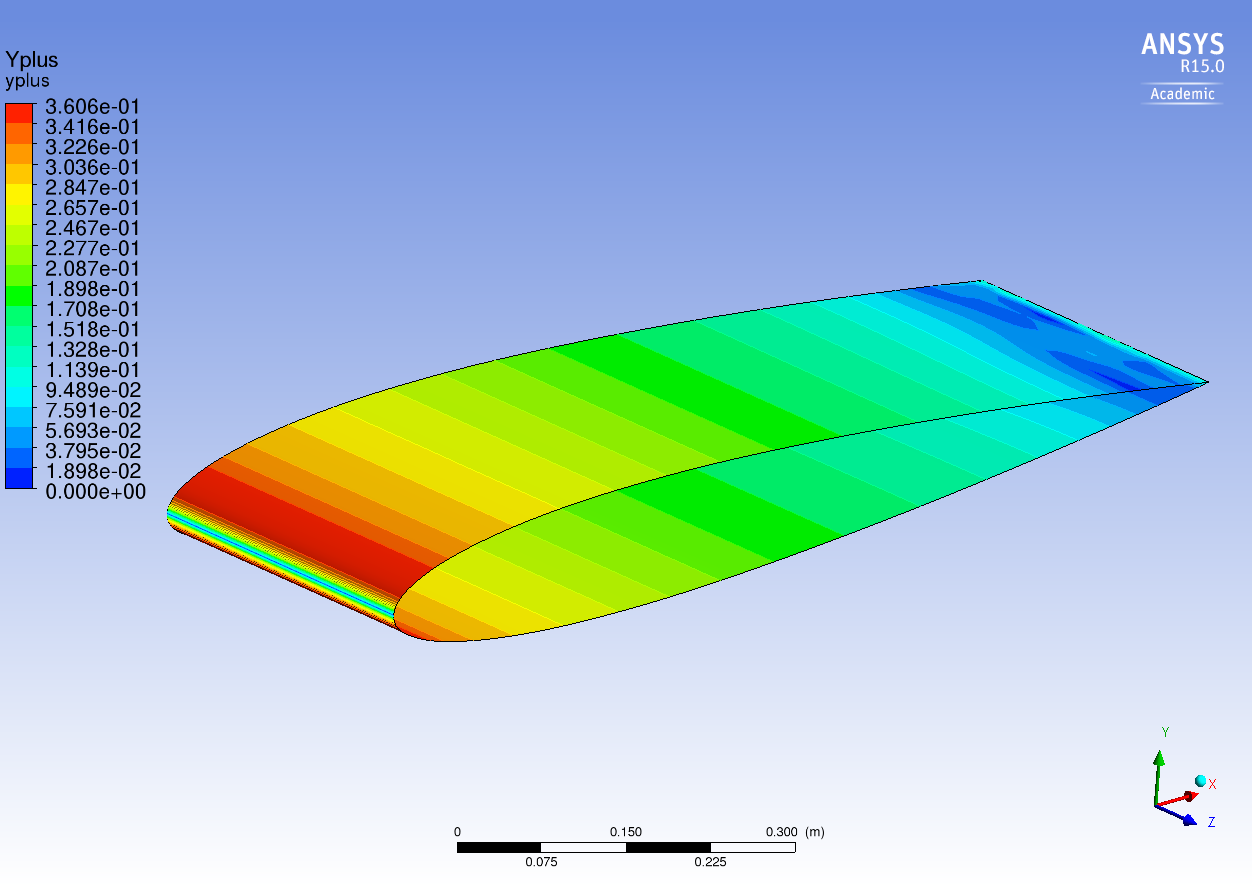
\includegraphics[scale=0.5]{yplus_on_airfoil.png}
\caption{The yplus value on the airfoil surface}
\label{yplus}
\end{figure}
%%
\section{Exporting data from Ansys CFX-Post}
For investigating the heat transfer a polyline was inserted exactly at the middle of the wing, in terms of depth in z-direction. The polyline was obtained by intersecting the wing surface with a xy-plane, which was inserted at 0.15m in z-direction. 
Subsequent the properties X-coordinate and Wall Heat Flux on this polyline were exported as csv file. This csv file was later as input for Matlab, which was used for plotting the data.

For comparison and evaluation purpose the same flow problem was simulated by Mr. Hassler as stationary simulation. The resolution file of this simulation was proceeded the same way, so that there could be exported a csv-file with the stationary data as well.
\section{Processing in MATLAB\textsuperscript{\textregistered}}
As next step the csv-files were imported into Matlab, where the data was extracted and used for plotting the wall heat flux over the wing length. For comparison reason both results, the stationary as well as the transient one, were displayed in the same plot, which can be seen in Figure 3.2. 

This data for the heat transfer was the basis for the calculation of diverse dimensionless numbers, which were of major importance for the evaluation of the simulation.
In detail, the Nußelt and the Froude number were used for comparison. For a cylinder the Froude number is more or less equal to one. This was utilized for the evaluation, since the nose of the airfoil can be compared to a cylinder.
The Nußelt and Froude number have been computed with three different approaches. For the first, the Nußelt number for a cylinder, equal to the airfoil nose diameter, was generated by means of the Prandtl and the Reynolds number with the relation given in equation ??. This was done for comparison reason and a typical specific heat transfer coefficient of 1,005 Joules per kilgram Kelvin was applied.
For the other two approaches the Nußelt number was computed from the values extracted from the simulation. Specificly the values of the wall heat flux at the stagnation point, where x is equal to zero, was of special interest. The stationary simulaton yielded a value of 253.69 Watt per square meter and the transient one a value of 257.05 Watt per square meter. These were used  for computating the heat transfer coefficient alpha, which can be obtained through the correlation
alpha = q / delta t, 
where delta t is the difference of the temperatures of the wall and the fluid. In this case it is one degree. With that and the airfoil nose diameter as specific length scale, given by
RE = ...,
the Nußelt number was calculated by means of equation ??.
In table ?? the differences and similarities of the single approaches can be observed.

